\section{Message Dissemination Model}
\label{sec:ode_model}
We investigate the selfish detection in this and the following sections.
Specifically, in this section, the ordinary differential equation model
is constructed to capture the state transition and the message dissemination
without detection and with complete detection.
\subsection{Case 1: without detection}
\label{subsec:wo_detc}
\begin{figure}
  \centering
  {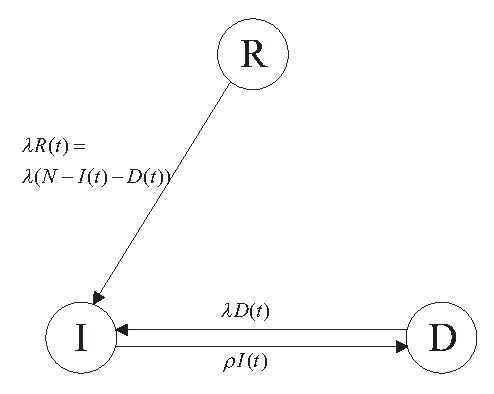
\includegraphics[width=0.23\textwidth]
  {fig/state_transition_no_detect.eps}}
     \caption{State transition of the relay nodes without detection.}
     \label{fig:ss_wo_dt}
\end{figure}
In the case without detection,
the relay node with message can become the selfish node,
but the selfish detection is not conducted by $src$.
Then the state transition is shown
in Fig.~\ref{fig:ss_wo_dt} with the following rules.
The nodes change from state $R$ to state $I$ if they contact $src$.
The corresponding incremental rate of state $I$ is $\lambda R(t)$ at time $t$.
Since the selfish node may also contact $src$ with the contact rate $\lambda$,
the rate of change from state $D$ to state $I$ is $\lambda D(t)$.
Because $N=R(t)+I(t)+D(t)$,
the total incremental rate of $I(t)$ is
$\lambda (R(t)+D(t))=\lambda (N-I(t))$.
Additionally, the rate of change from state $I$ to state $D$ is $\rho I(t)$.
We can obtain the derivative of $I(t)$ with respect to time $t$,
$\frac{\mathrm{d} I(t)}{\mathrm{d} t} = \lambda (N-I(t)) - \rho I(t)$.
Similar to $\frac{\mathrm{d} I(t)}{\mathrm{d} t}$,
we can get the derivative of $D(t)$
and the derivative of $R(t)$ respectively,
i.e., $\frac{\mathrm{d} D(t)}{\mathrm{d} t}$ and
$\frac{\mathrm{d} R(t)}{\mathrm{d} t}$.
Thus the state transition can be represented as
\begin{small}
\begin{equation}
\label{eq:IDR_wo}
\begin{aligned}
\frac{\mathrm{d} I(t)}{\mathrm{d} t} &=  \lambda (N-I(t)) - \rho I(t),\\
\frac{\mathrm{d} D(t)}{\mathrm{d} t} &= - \lambda D(t) + \rho I(t),\\
\frac{\mathrm{d} R(t)}{\mathrm{d} t} &= - \lambda (N-I(t)-D(t)).
\end{aligned}
\end{equation}
\end{small}
Since $I(t)$ in (\ref{eq:IDR_wo}) is formed by the first-order first-power
ordinary differential equations (ODE)~\cite{CC2007PerfAnaly},
we can obtain the general solutions of $I(t)$, that is,
\begin{small}
\begin{equation}
\nonumber
\begin{aligned}
I(t) = C_{I} e^{-(\lambda + \rho)t} + \frac{ \lambda N }{ \lambda + \rho }.
\end{aligned}
\end{equation}
\end{small}
Note that $I(0)=0$, $D(0)=0$ and $R(0)=N$,
which means only $src$ carries the message at time $0$.
Thus $C_{I} = \frac{ -\lambda N }{ \lambda + \rho }$, and
\begin{small}
\begin{equation}
\nonumber
\begin{aligned}
I(t) = \frac{ \lambda N }{ \lambda + \rho }(1- e^{-(\lambda + \rho)t}),
\end{aligned}
\end{equation}
\end{small}
where $0 \le t \le T$.
Similarly, we can calculate the general solution of the first-order ODE $D(t)$
from $\frac{\mathrm{d} D(t)}{\mathrm{d} t} + \lambda D(t) = \rho I(t)$,
\begin{small}
\begin{equation}
\label{eq:D_formula}
\begin{aligned}
D(t) &= C_{D} e^{-\int \lambda dt} + e^{-\int \lambda dt} \int \rho I(t) e^{\int \lambda dt} dt \\
%&= C_{D} e^{- \lambda t} +
%e^{- \lambda t} \int \rho \frac{ \lambda N }{ \lambda + \rho } (1 - e^{-(\lambda + \rho)t}) e^{ \lambda t} dt \\
&= C_{D} e^{- \lambda t} + \frac{ \lambda N }{ \lambda + \rho } e^{-(\lambda + \rho)t} + \frac{ \rho N }{ \lambda + \rho }.
\end{aligned}
\end{equation}
\end{small}
Because of $D(0)=0$,
\begin{small}
\begin{equation}
\nonumber
\begin{aligned}
D(t) &= -N e^{- \lambda t} + \frac{ \lambda N }{ \lambda + \rho } e^{-(\lambda + \rho)t} + \frac{ \rho N }{ \lambda + \rho }.
\end{aligned}
\end{equation}
\end{small}
Since $I(t)+D(t)+R(t)=N$, $0 \le t \le T$,
$R(t)$ can be computed based on the solved solution of $I(t)$ and $D(t)$.
Thus the solution of (\ref{eq:IDR_wo}) can be derived as
\begin{small}
\begin{equation}
\label{eq:IDR_wo_solu}
\begin{aligned}
I(t) &= \frac{ \lambda N }{ \lambda + \rho }(1- e^{-(\lambda + \rho)t}), \\
D(t) &= N (\frac{\lambda e^{-(\lambda + \rho)t} + \rho}{ \lambda + \rho } - e^{- \lambda t}), \\
R(t) &= N e^{- \lambda t},
\end{aligned}
\end{equation}
\end{small}
which depicts the change of the states when the time ranges from $0$ to $T$.
And $I(t)$, $D(t)$, $R(t)$ $\ge 0$ always hold when $t \ge 0$.
From the solutions of $I(t)$, $D(t)$ and $R(t)$,
we can find that $I(t) \rightarrow \frac{ \lambda N }{ \lambda + \rho }$,
$D(t) \rightarrow \frac{ \rho N }{ \lambda + \rho }$
and $R(t) \rightarrow 0$,
when $t \rightarrow + \infty$.
To verify the validity of the ODE model (\ref{eq:IDR_wo}),
we conduct the simulations with randomly settings.
The corresponding results are presented in Section.~\ref{subsec:pe_valid}.

The cost $J$ in (\ref{eq:obj}) also can be calculated based on (\ref{eq:IDR_wo_solu}).
Note that $U(t)=0$, $\forall t$,
in the case without detection.
$J$ is determined by the expected number of selfish nodes $D(t)$,
$0 \le t \le T$,
which is proportional to the reward consumed by selfish behaviors.
Thus $J$ can be computed as
\begin{small}
\begin{equation}
\label{eq:IDR_wo_J}
\begin{aligned}
J &= \int_{0}^{T} (1-\alpha) D(t) dt, \\
&= \int_{0}^{T} (1-\alpha) N (\frac{\lambda e^{-(\lambda + \rho)t} + \rho}{ \lambda + \rho } - e^{- \lambda t}) dt, \\
&= N (1-\alpha) \left( \frac{\lambda (1-e^{-(\lambda+\rho)T})}{ (\lambda + \rho)^{2} }
+ \frac{\rho T}{\lambda + \rho}
- \frac{1-e^{-\lambda T}}{\lambda} \right).
\end{aligned}
\end{equation}
\end{small}
Similarly, we can get the total paid reward in this case
\begin{small}
\begin{equation}
\nonumber
\begin{aligned}
P &= \beta \int_{0}^{T} I(t) + D(t) dt
%&= \beta \int_{0}^{T} (N - N e^{- \lambda t}) dt, \\
= N \beta (T - \frac{ 1 - e^{-\lambda T} }{\lambda} ).
\end{aligned}
\end{equation}
\end{small}
Furthermore, the fraction between the wasted reward and the total paid reward can be obtained as
\begin{small}
\begin{equation}
\nonumber
\begin{aligned}
p = \frac{\int_{0}^{T} D(t) dt}{\int_{0}^{T} I(t) + D(t) dt}
&= \frac{ \frac{\lambda (1-e^{-(\lambda+\rho)T})}{ (\lambda + \rho)^{2} }
+ \frac{\rho T}{\lambda + \rho}
- \frac{1-e^{-\lambda T}}{\lambda} }
{T - \frac{ 1 - e^{-\lambda T} }{\lambda} }.
\end{aligned}
\end{equation}
\end{small}

\subsection{Case 2: with complete detection}
\label{subsec:full_detc}
\begin{figure}
  \centering
  {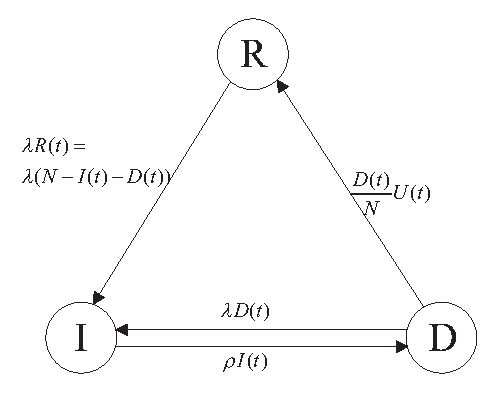
\includegraphics[width=0.23\textwidth]
  {fig/state_transition_detect.eps}}
     \caption{State transition of the relay nodes.}
     \label{fig:ss_dt}
\end{figure}
In the case with complete detection,
$src$ conducts the selfish node detection in the whole message lifetime.
The detections are conducted at
time {$T_{m}$, $2 T_{m}$, $\cdots$, $k T_{m}$},
where $k T_{m} \le T < (k+1) T_{m}$.
In every detection, a randomly selected node $n_{i}$
is checked by $src$ whether $n_{i}$ is a selfish node.
We can find that the decrement of selfish node number
only occurs at the instant $iT_{m}$
in the case with complete detection.

In order to simplify the model,
we exploit a continuous manner to
describe this case with complete detection.
Considering that the checked relay node
is randomly selected from the $N$ node set,
we calculate the probability of selecting a selfish node
as $\frac{D(t)}{N}$.
Since the detection rate is constrained by $U(t)$,
we let $\frac{D(t)}{N}U(t)$ denote
the change rate from state $D$ to state $R$ caused by detections.
Thus the state transition of the fully detection case
is constructed as Fig.~\ref{fig:ss_dt}.
The approximate model of the state transition in the case with complete detection
will be constructed as
\begin{small}
\begin{equation}
\label{eq:IDR_full}
\begin{aligned}
\frac{\mathrm{d} I(t)}{\mathrm{d} t} &=  \lambda (N-I(t)) - \rho I(t),\\
\frac{\mathrm{d} D(t)}{\mathrm{d} t} &= - \lambda D(t) + \rho I(t) - \frac{D(t)}{N} U(t),\\
\frac{\mathrm{d} R(t)}{\mathrm{d} t} &= - \lambda (N-I(t)-D(t)) + \frac{D(t)}{N} U(t),
\end{aligned}
\end{equation}
\end{small}
based on the model in the case without detection (\ref{eq:IDR_wo}).
Here $U(t) = U_{m}$, $\forall t$, $0 \le t \le T$.
The initial state is that $I(0)=D(0)=0$ and $R(0)=N$.
So the solution of $I(t)$, which does not change from $(\ref{eq:IDR_wo_solu})$,
is that $I(t) = \frac{ \lambda N }{ \lambda + \rho }(1- e^{-(\lambda + \rho)t})$.
From $\frac{\mathrm{d} D(t)}{\mathrm{d} t} + (\lambda + \frac{U_{m}}{N}) D(t)= \rho I(t)$,
we can derive that
\begin{small}
\begin{equation}
\nonumber
\begin{aligned}
& D(t) \\
=& C_{2D} e^{\int -(\lambda + \frac{U_{m}}{N}) dt}
+ e^{\int -(\lambda + \frac{U_{m}}{N}) dt} \int \rho I(t) e^{\int (\lambda + \frac{U_{m}}{N}) dt} dt \\
=& C_{2D} e^{-(\lambda + \frac{U_{m}}{N})t}
- \frac{ \rho \lambda N }{ (\lambda + \rho)(\frac{U_{m}}{N} - \rho) } e^{-(\lambda + \rho)t}
+ \frac{ \rho \lambda N }{ (\lambda + \rho)(\lambda + \frac{U_{m}}{N}) }.
\end{aligned}
\end{equation}
\end{small}
Since $D(0) = 0$ and $I(t) + D(t) + R(t) = N$,
%\begin{small}
%\begin{equation}
%\nonumber
%\begin{aligned}
%D(t) =& \frac{ \rho \lambda N }{ \lambda + \rho } \frac{1}{\lambda + \frac{U_{m}}{N}}
%- \frac{\rho \lambda N}{(\lambda + \frac{U_{m}}{N})(\frac{U_{m}}{N} - \rho)}  e^{-(\lambda + \frac{U_{m}}{N})t}\\
%& - \frac{ \rho \lambda N }{ \lambda + \rho } \frac{1}{\frac{U_{m}}{N} - \rho} e^{-(\lambda + \rho)t}
%\end{aligned}
%\end{equation}
%\end{small}
the solution of (\ref{eq:IDR_full}) can be calculated as
\begin{small}
\begin{equation}
\label{eq:IDR_full_solu}
\begin{aligned}
I(t) =& \frac{ \lambda N }{ \lambda + \rho }(1- e^{-(\lambda + \rho)t}),\\
D(t) =& \frac{ \rho \lambda N }{ (\lambda + \rho)(\lambda + \frac{U_{m}}{N}) }
+ \frac{\rho \lambda N}{(\lambda + \frac{U_{m}}{N})(\frac{U_{m}}{N} - \rho)}  e^{-(\lambda + \frac{U_{m}}{N})t}\\
& - \frac{ \rho \lambda N }{ (\lambda + \rho)(\frac{U_{m}}{N} - \rho) } e^{-(\lambda + \rho)t},\\
R(t) =& N - \frac{ \lambda N }{ \lambda + \rho } \left( \frac{\rho}{\lambda + \frac{U_{m}}{N}} + 1 \right)
+ \frac{ \lambda U_{m} }{ (\lambda + \rho)(\frac{U_{m}}{N} - \rho) } e^{-(\lambda + \rho)t}\\
& - \frac{\rho \lambda N}{(\lambda + \frac{U_{m}}{N})(\frac{U_{m}}{N} - \rho)}  e^{-(\lambda + \frac{U_{m}}{N})t}.
\end{aligned}
\end{equation}
\end{small}
We can find that $I(t) \rightarrow \frac{ \lambda N }{ \lambda + \rho }$,
$D(t) \rightarrow \frac{ \rho \lambda N }{ (\lambda + \rho)(\lambda + \frac{U_{m}}{N}) }$,
and $R(t) \rightarrow  N - \frac{ \lambda N }{ \lambda + \rho } \left( \frac{\rho}{\lambda + \frac{U_{m}}{N}} + 1 \right)$
when $t \rightarrow +\infty$ according to (\ref{eq:IDR_full_solu}).
Here $R(+\infty) \neq 0$ in the steady state
is caused by the complete selfish detection.
Based on the approximate model (\ref{eq:IDR_full})
and the corresponding solutions (\ref{eq:IDR_full_solu}),
the estimation of the total cost $\hat{J}$
can be computed as
\begin{small}
\begin{equation}
\label{eq:IDR_full_J}
\begin{aligned}
\hat{J} =& \int_{0}^{T} (1-\alpha) D(t) + \alpha U(t) dt, \\
=& \frac{ (1-\alpha) \rho \lambda N T }{ (\lambda + \rho)(\lambda + \frac{U_{m}}{N}) }
- \frac{(1-\alpha) \rho \lambda N}{ {(\lambda + \frac{U_{m}}{N})}^{2} (\frac{U_{m}}{N} - \rho)}
(e^{-(\lambda + \frac{U_{m}}{N})T} - 1 ) \\
&+ \frac{(1-\alpha) \rho \lambda N }{ {(\lambda + \rho)}^{2} (\frac{U_{m}}{N} - \rho) }
(e^{-(\lambda + \rho)T} - 1 )
+ \alpha T U_{m}.
\end{aligned}
\end{equation}
\end{small}
The reason why (\ref{eq:IDR_full_J}) is the estimation of the cost
is that the decrement of $D(t)$ actually occurs in the end of the detection cycle.
However, the change rate of $D(t)$ in (\ref{eq:IDR_full})
is denoted by $\frac{D(t)}{N}U(t)$ in the above analysis.
So there exists a deviation between the true cost $J$ and the estimated cost $\hat{J}$
<<<<<<< HEAD
in the case with fully detection.
\begin{lem}\label{lem_1}
Let $D(t)$
=======
in the case with complete detection.
\begin{lem}
>>>>>>> 5df34e4a02464f9c5ee16f8b228c71d6cc464e41
When $t \rightarrow +\infty$, $T_{m} \ll T$,
a deviation between $D(t)$ in the approximate model (\ref{eq:IDR_full_solu})
and in the real scenario is limited.
\end{lem}

\begin{proof}
At first we discuss the real scenario of the complete detection case.
Without loss of generality,
assume that $(0, T)$ can be divided into $k$ detection cycles
and a following duration $t_{k+1}$.
Here the $i$-th detection cycle is denoted by $(t_{i-1}, t_{i}]$,
where $t_{i} - t_{i-1} = T_{m}$ and $t_{k+1} < T_{m}$.
In every detection cycle,
$D(t)$ increases from $D(t_{i-1})$ to $D(t_{i}^{-})$
in $(t_{0}, t_{1}^{-})$.
Since the detection occurs at the instant $t_{i}$,
$D(t_{i}^{+}) = \frac{N-1}{N}D(t_{i}^{-})$.
From (\ref{eq:IDR_wo_solu}) we can find that $D(t)$ increases with time in the case
and approaches to the stable state in the case without detection.
In the case with complete detection,
when $t \rightarrow +\infty$,
$D(t)$ also approaches to the stable state,
where $D(t_{i-1}^{+}) = D(t_{i}^{+})$.
We can obtain that
\begin{small}
\begin{equation}
\nonumber
\begin{aligned}
D(t_{i-1}^{+}) = & C_{i} e^{-\lambda t_{i-1}^{+}}
+ \frac{\lambda N}{\lambda + \rho} e^{-(\lambda+\rho)t_{i-1}^{+}}
+ \frac{\rho N}{\lambda+\rho}, \\
D(t_{i}^{-}) = & C_{i} e^{-\lambda t_{i}^{+}}
+ \frac{\lambda N}{\lambda + \rho} e^{-(\lambda+\rho)t_{i}^{+}}
+ \frac{\rho N}{\lambda+\rho},
\end{aligned}
\end{equation}
\end{small}
in $(t_{i-1}, t_{i})$ based on (\ref{eq:D_formula}).
Then, when $i \rightarrow +\infty$,
\begin{small}
\begin{equation}
\nonumber
\begin{aligned}
D(t_{i}^{+}) =& \frac{N-1}{N} D(t_{i}^{-}) \\
=& \frac{N-1}{N} D(t_{i-1}^{+}) e^{-\lambda T_{m}}
+ \frac{\rho (N-1)}{\lambda + \rho} (1 - e^{-\lambda T_{m}})
\end{aligned}
\end{equation}
\end{small}
Considering that $D(t_{i-1}^{+}) = D(t_{i}^{+})$, we can get that
\begin{small}
\begin{equation}
\nonumber
\begin{aligned}
\lim_{i \rightarrow +\infty} D(t_{i}^{+}) &=
\frac{\rho(N-1)}{\lambda+\rho} \frac{1 - e^{-\lambda T_{m}}}
{(1 - \frac{N-1}{N}e^{-\lambda T_{m}})} \\
\lim_{i \rightarrow +\infty} D(t_{i}^{-}) &=
\frac{\rho N}{\lambda+\rho} \frac{1 - e^{-\lambda T_{m}}}
{(1 - \frac{N-1}{N}e^{-\lambda T_{m}})} \\
\end{aligned}
\end{equation}
\end{small}
According to (\ref{eq:IDR_full_solu}),
$D(+\infty) = \frac{\rho \lambda N}
{(\lambda + \rho)(\lambda + \frac{U_{m}}{N})}$.
Since these limitations are the limited values related to
$\rho$, $\lambda$, $N$ and $U_{m}$,
the deviation of $D(t)$ between in the approximate model and in the real scenario is limited.
\end{proof}

\begin{lem}
Let $J$ denote the cost in the complete detection case.
In the case with fully detection,
$|J - \hat{J}|$ is less than $(1-\alpha) T N$.
\end{lem}
\begin{proof}
Considering that $U(t) = \hat{U}(t) = U_{m}$,
we can derive that $\int_{0}^{T} U(t) dt = T U_{m} = \int_{0}^{T} \hat{U}(t) dt $.
And the deviation between the estimated cost and the true cost
\begin{small}
\begin{equation}
\label{eq:delta_J}
\begin{aligned}
|J - \hat{J}| = & \left| \int_{0}^{T} (1-\alpha)D(t) dt - \int_{0}^{T} (1-\alpha) \hat{D(t)} dt \right| \\
\le & (1-\alpha) \int_{0}^{T} |(D(t)-\hat{D(t)})| dt \\
\le & (1-\alpha) T N
\end{aligned}
\end{equation}
\end{small}
where $0 \le D(t), \hat{D(t)} \le N$.

\end{proof}

We also can compute the approximate total reward is
\begin{small}
\begin{equation}
\nonumber
\begin{aligned}
\hat{P} &= \beta \int_{0}^{T} I(t) + D(t) dt, \\
& = \frac{\beta \rho \lambda N T}{ (\lambda + \rho)(\lambda + \frac{U_{m}}{N}) }
- \frac{\beta \rho \lambda N}{ {(\lambda + \frac{U_{m}}{N})}^{2} (\frac{U_{m}}{N} - \rho)}
(e^{-(\lambda + \frac{U_{m}}{N})T} - 1 ) \\
&+ \frac{\beta \rho \lambda N }{ {(\lambda + \rho)}^{2} (\frac{U_{m}}{N} - \rho) }
(e^{-(\lambda + \rho)T} - 1 ) 
+ \frac{ \lambda N }{ (\lambda + \rho)^2 } (e^{-(\lambda + \rho)T} - 1 ) \\
& + \frac{ \beta \lambda N T }{ \lambda + \rho }
\end{aligned}
\end{equation}
\end{small}
Similarly, the utilization ratio of reward also can be obtained
$\hat{p} = \frac{\int_{0}^{T} D(t) dt}{\int_{0}^{T} I(t) + D(t) dt}$.
From (\ref{eq:IDR_full_solu}) to (\ref{eq:IDR_wo_solu}),
we find $I(t)$ does not change but $D(t)$ decreases.
Thus this complete detection case can reduce the selfish behaviors
with the additional cost of the selfish node detections,
e.g., energy, bandwidth and wireless communication fee.
Thus we try to achieve the tradeoff between the paid reward and the detection cost
via the optimal solution.